\chapter{Módulos e Funcionalidades do Frontend}

O frontend do sistema BusLy oferece uma interface moderna e intuitiva para gestão completa de operações de transporte rodoviário. A aplicação é desenvolvida em Next.js~15 com React~19, proporcionando uma experiência de usuário fluida e responsiva.

\section{Autenticação e Gestão de Empresa}

\subsection{Tela de Login e Registro}

A autenticação do sistema é realizada através de uma interface limpa e moderna. A tela de login apresenta campos para email e senha, com validação em tempo real e feedback visual para o usuário. O sistema utiliza NextAuth v4 para gerenciamento de sessão, garantindo segurança e persistência do estado de autenticação.

\begin{figure}[H]
  \centering
  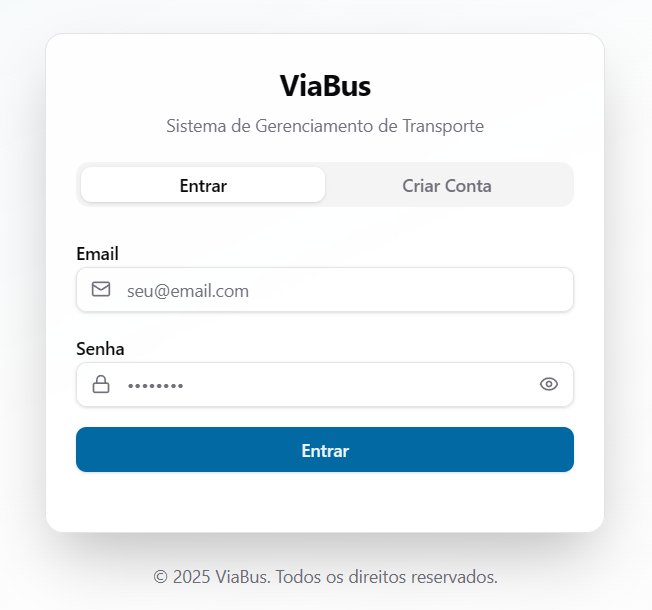
\includegraphics[width=0.8\textwidth]{imagens/tela-login.png}
  \caption{Tela de login do sistema BusLy.}
  \label{fig:tela-login}
\end{figure}

\subsection{Fluxo de Criação da Empresa}

Após o primeiro acesso, usuários sem empresa associada são direcionados para o fluxo de criação de empresa. Este processo inclui cadastro da empresa com informações básicas (nome, CNPJ, endereço), configuração inicial de parâmetros operacionais e validação automática de dados.

\begin{figure}[H]
  \centering
  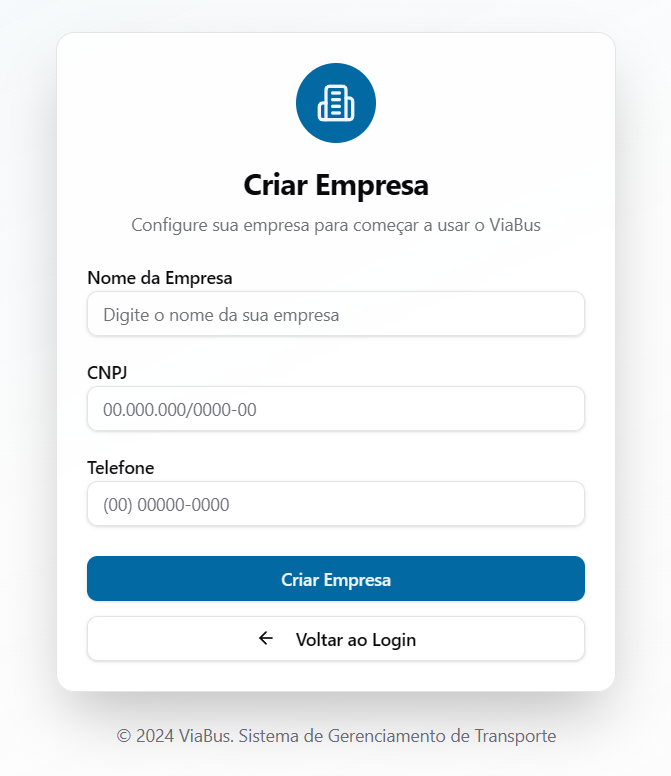
\includegraphics[width=0.8\textwidth]{imagens/criacao-empresa.png}
  \caption{Formulário de criação de empresa.}
  \label{fig:criacao-empresa}
\end{figure}

\section{Painel de Controle (Dashboard)}

O dashboard principal oferece uma visão consolidada das operações da empresa, apresentando métricas importantes e acesso rápido aos módulos principais.

\subsection{Visão Geral}

O painel de controle exibe cards informativos com estatísticas em tempo real: total de viagens, passagens vendidas, veículos ativos, motoristas disponíveis, rotas ativas e paradas cadastradas.

\begin{figure}[H]
  \centering
  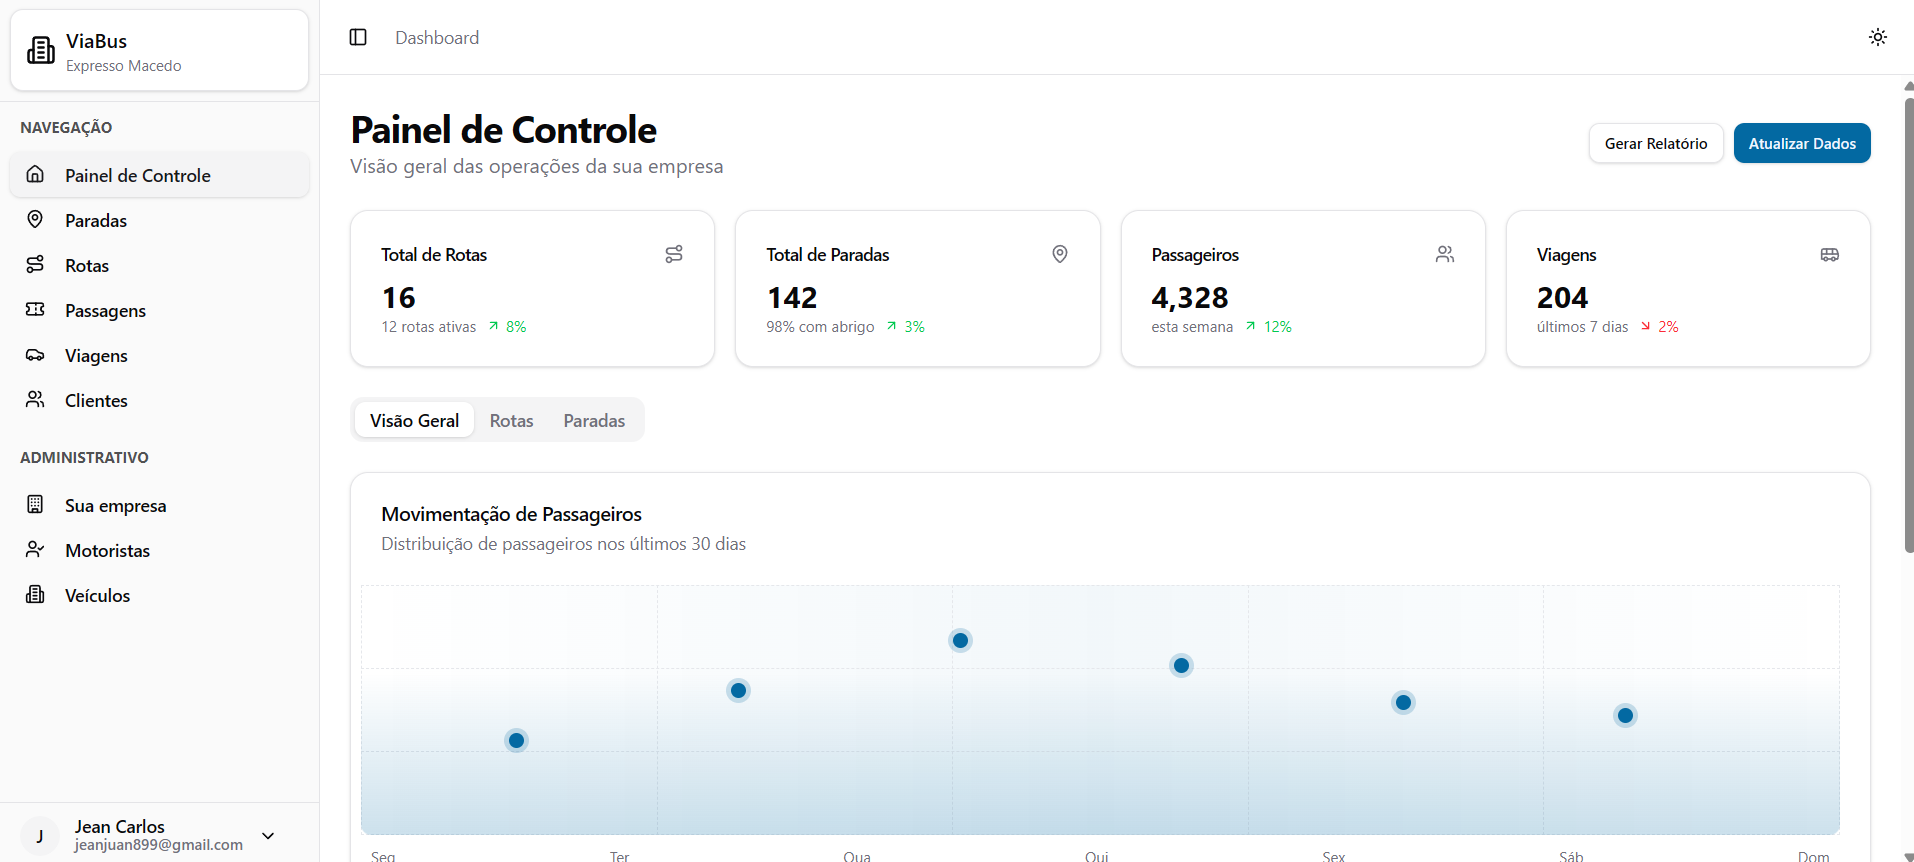
\includegraphics[width=0.9\textwidth]{imagens/dashboard.png}
  \caption{Painel de controle principal com métricas e navegação.}
  \label{fig:dashboard}
\end{figure}

\section{Módulo de Paradas}

O módulo de paradas permite o cadastro e gerenciamento de pontos de embarque e desembarque, com integração a mapas interativos.

\subsection{Listagem de Paradas}

A tela de listagem apresenta todas as paradas cadastradas em formato de tabela, com funcionalidades de busca, filtros e ações rápidas (editar, visualizar, excluir).

\begin{figure}[H]
  \centering
  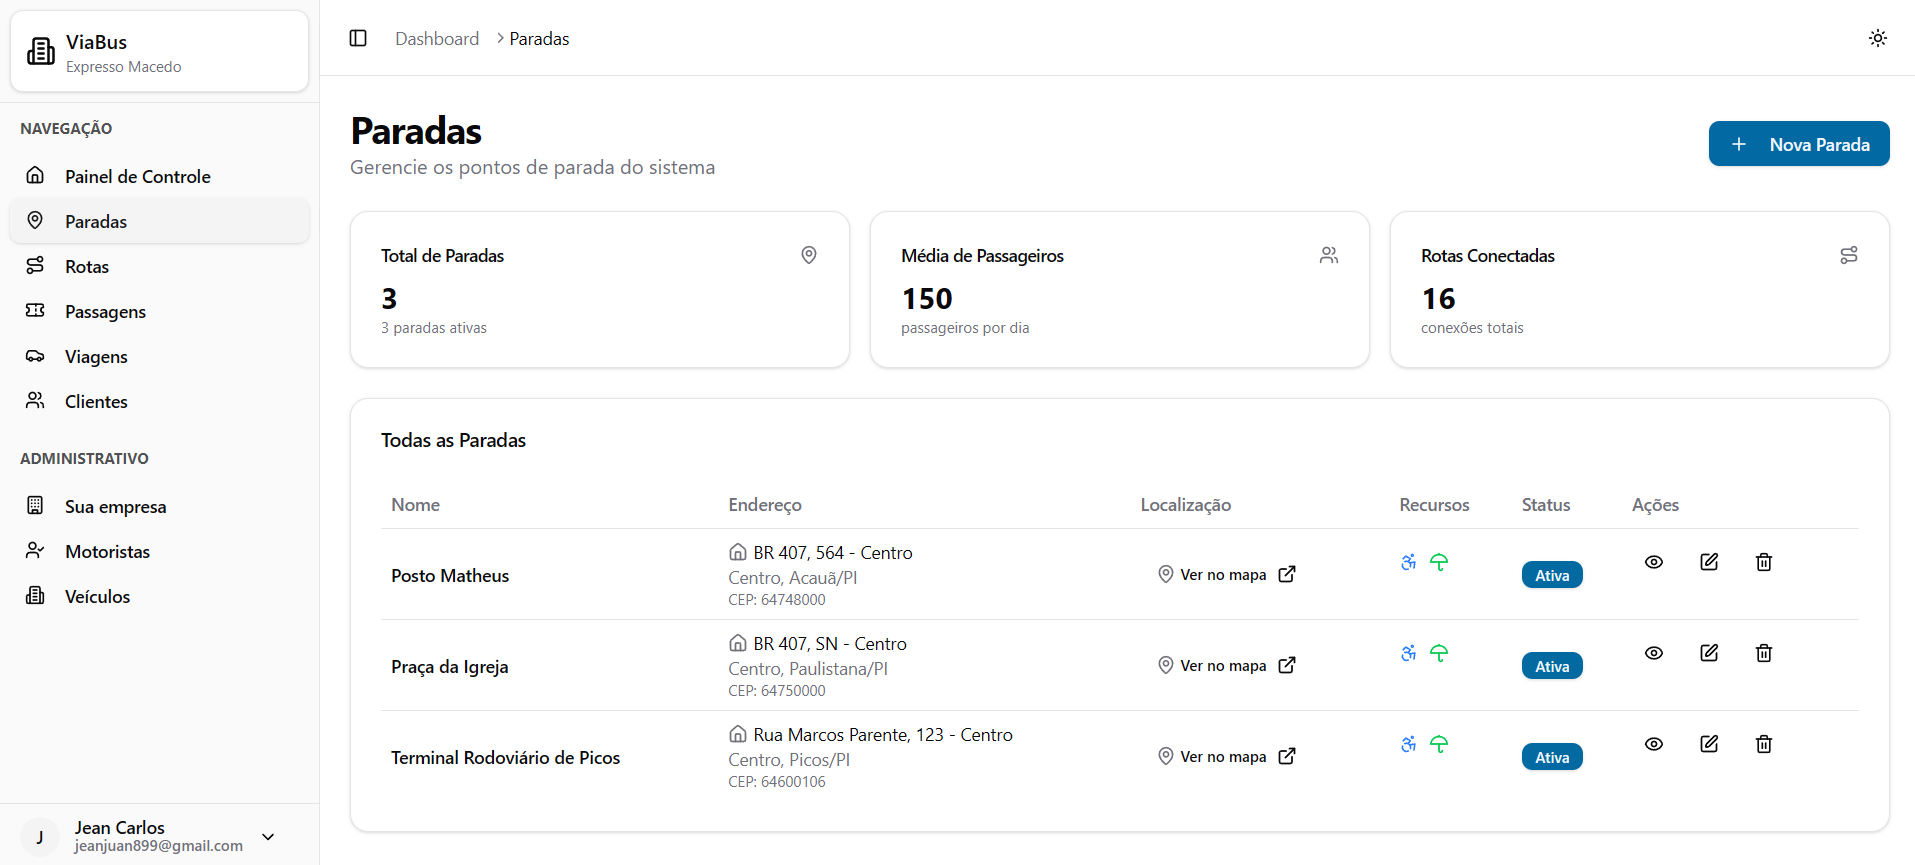
\includegraphics[width=0.9\textwidth]{imagens/listagem-paradas.png}
  \caption{Listagem de paradas com funcionalidades de busca e filtros.}
  \label{fig:listagem-paradas}
\end{figure}

\subsection{Criação e Edição de Paradas}

O formulário de cadastro de paradas integra um mapa interativo baseado em Leaflet, permitindo seleção geográfica por clique, arrastar marcador para ajuste fino, validação de endereço e informações detalhadas como nome, descrição e horários de funcionamento.

\begin{figure}[H]
  \centering
  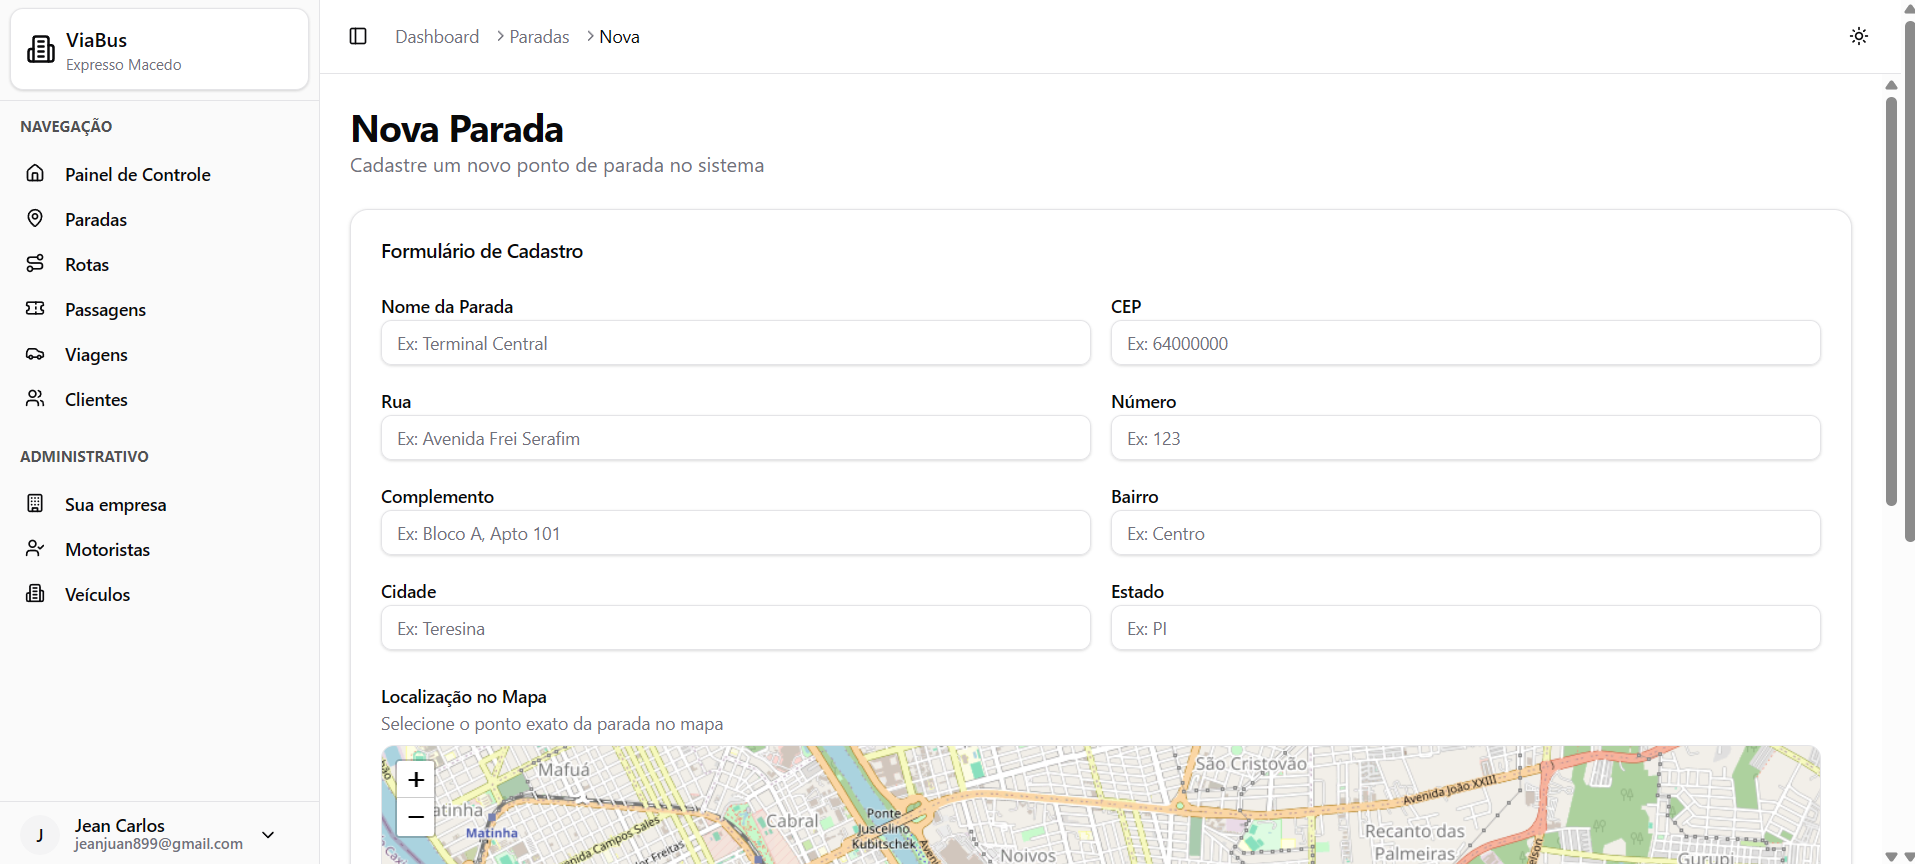
\includegraphics[width=0.9\textwidth]{imagens/formulario-parada.png}
  \caption{Formulário de cadastro de parada com mapa interativo.}
  \label{fig:formulario-parada}
\end{figure}

\section{Módulo de Rotas}

O módulo de rotas permite a criação de itinerários conectando paradas em sequência lógica, incluindo definição de paradas em ordem de visitação, cálculo automático de distâncias e configuração de preços por trecho.

\begin{figure}[H]
  \centering
  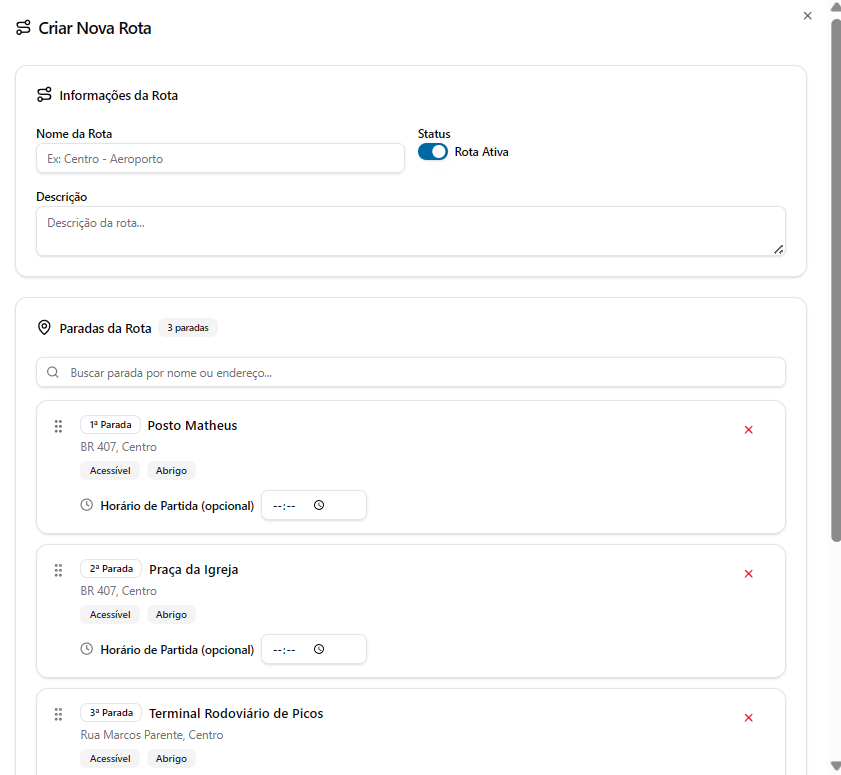
\includegraphics[width=0.9\textwidth]{imagens/criacao-rota.png}
  \caption{Interface de criação de rota com seleção de paradas.}
  \label{fig:criacao-rota}
\end{figure}

\section{Módulo de Veículos}

O módulo de veículos gerencia a frota da empresa, permitindo cadastro completo (placa, modelo, capacidade, ano), controle de status operacional (ativo, em manutenção, inativo), histórico de viagens e filtros avançados.

\begin{figure}[H]
  \centering
  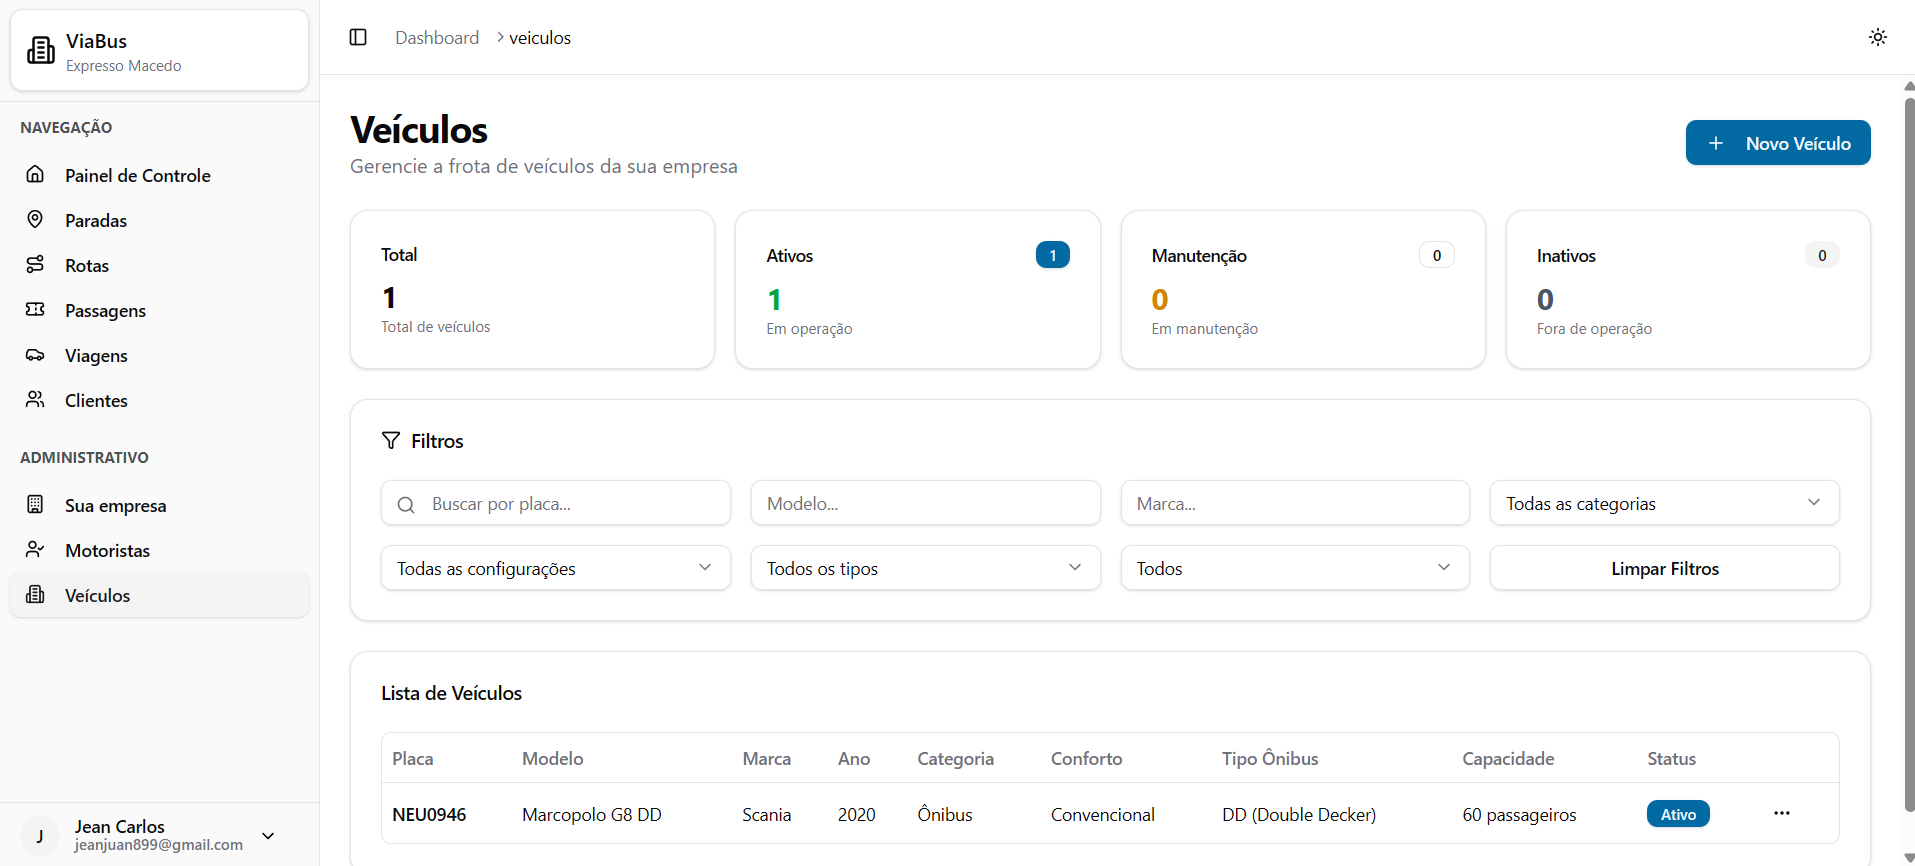
\includegraphics[width=0.9\textwidth]{imagens/veiculos.png}
  \caption{Listagem de veículos com status operacional.}
  \label{fig:veiculos}
\end{figure}

\section{Módulo de Motoristas}

O módulo de motoristas gerencia a equipe de condutores, incluindo dados pessoais (nome, CPF, CNH, contatos), informações profissionais (categoria da CNH, experiência), status de disponibilidade e histórico de viagens.

\begin{figure}[H]
  \centering
  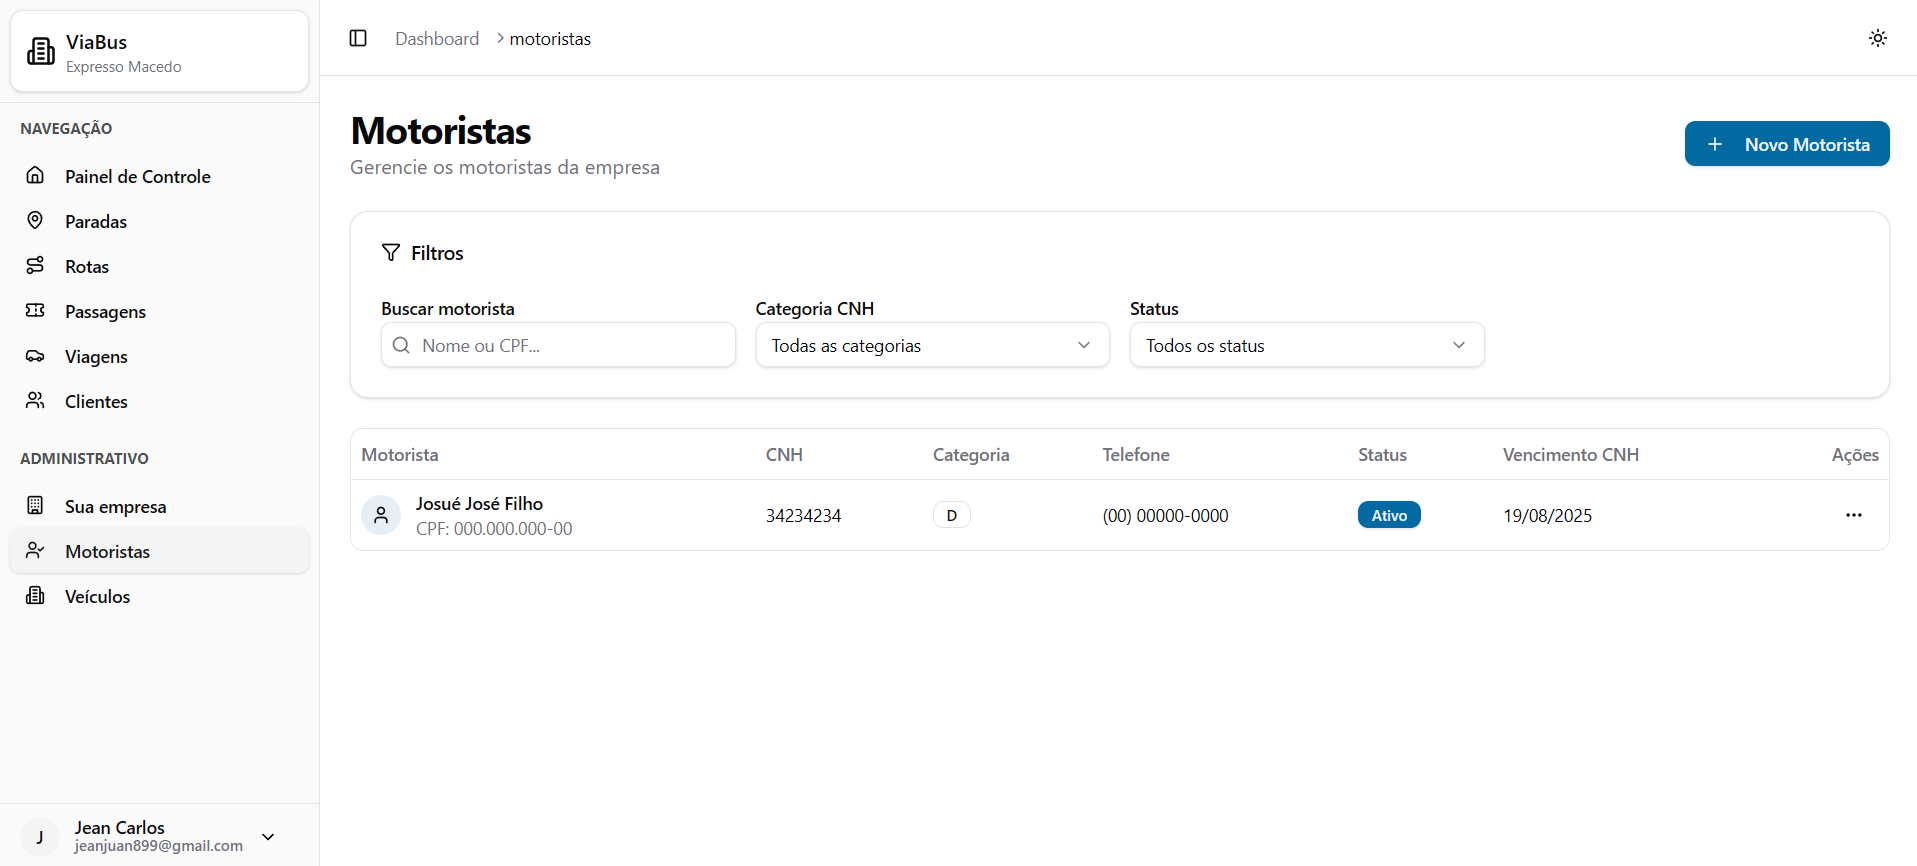
\includegraphics[width=0.9\textwidth]{imagens/motoristas.png}
  \caption{Interface de gerenciamento de motoristas.}
  \label{fig:motoristas}
\end{figure}

\section{Módulo de Viagens}

O módulo de viagens permite o agendamento e gerenciamento de viagens através de um fluxo estruturado: seleção da rota, definição de data e horário, associação de veículo, designação de motorista, configuração de preços e confirmação final.

\begin{figure}[H]
  \centering
  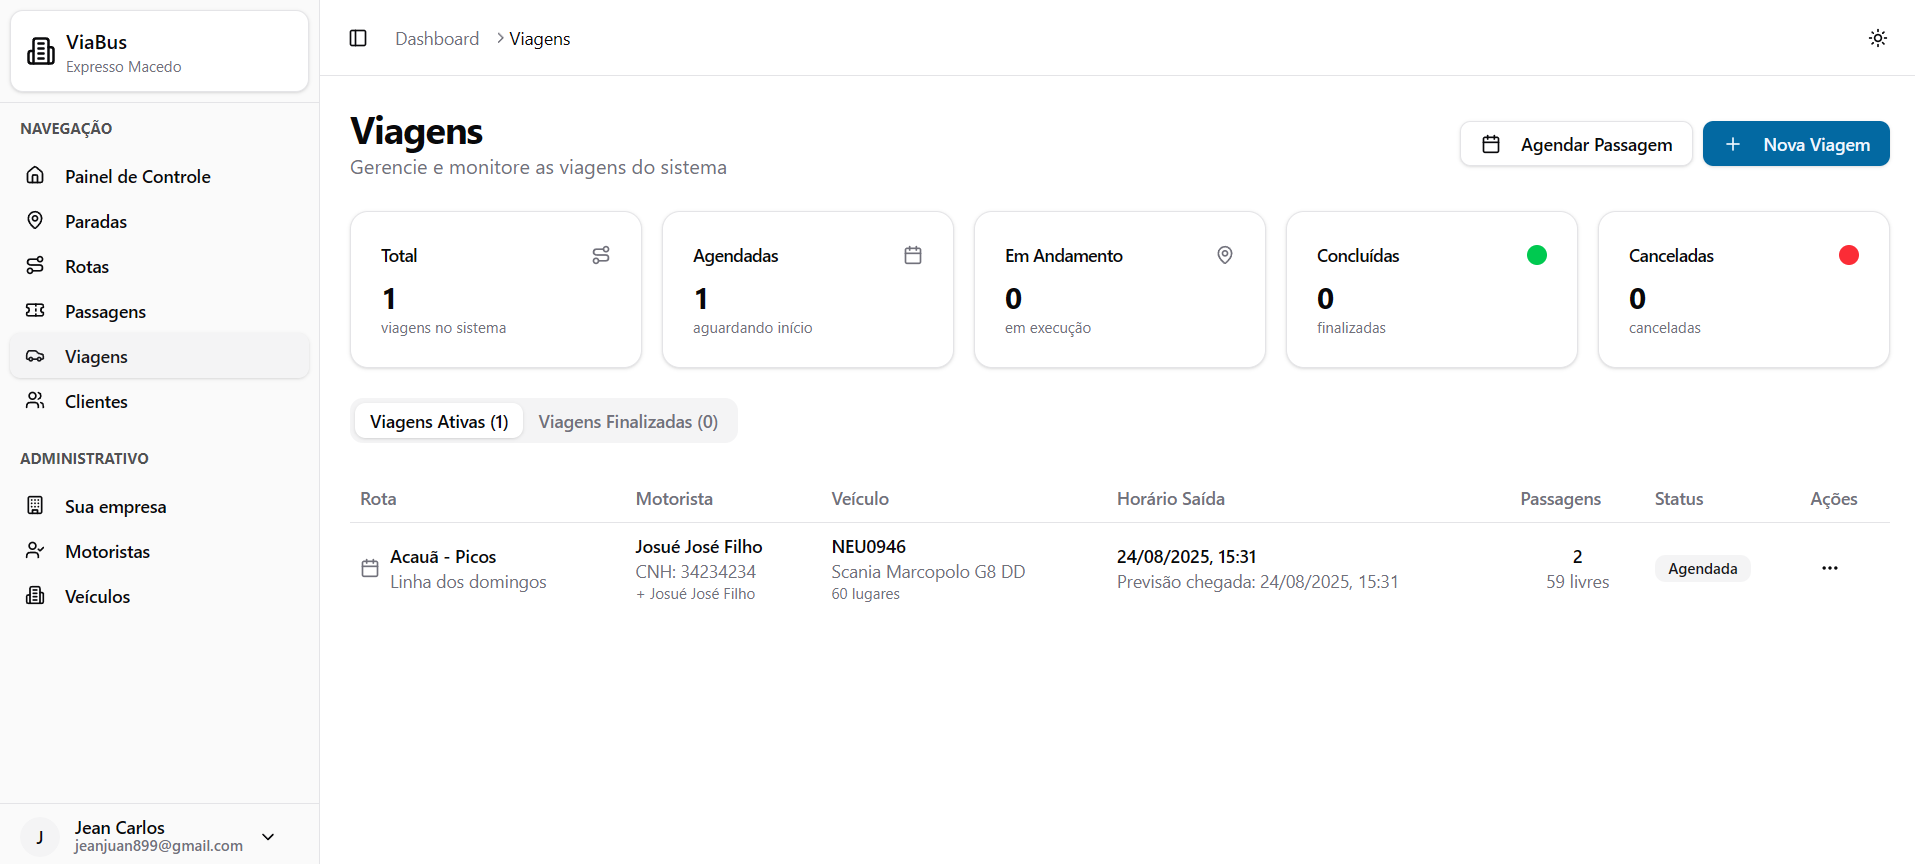
\includegraphics[width=0.9\textwidth]{imagens/agendamento-viagem.png}
  \caption{Processo de agendamento de viagem.}
  \label{fig:agendamento-viagem}
\end{figure}

\section{Módulo de Venda de Passagens}

O módulo de passagens implementa um assistente (wizard) intuitivo para venda de passagens, guiando o usuário através de cinco etapas sequenciais.

\subsection{Assistente de Venda de Passagens}

\subsubsection{1. Seleção de Rota}

Primeira etapa com listagem de rotas disponíveis, filtros por data, informações da rota (paradas, horários, preços) e verificação de disponibilidade de assentos.

\begin{figure}[H]
  \centering
  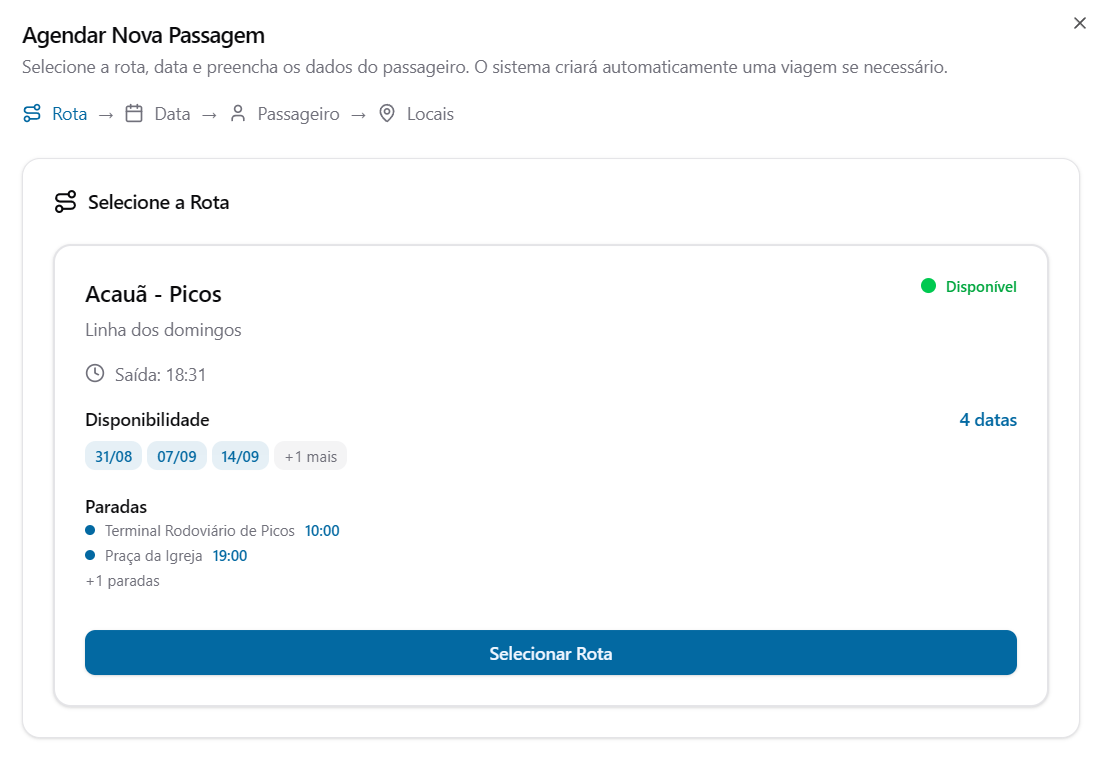
\includegraphics[width=0.9\textwidth]{imagens/wizard-rota.png}
  \caption{Seleção de rota no wizard de passagens.}
  \label{fig:wizard-rota}
\end{figure}

\subsubsection{2. Seleção de Data e Horário}

Segunda etapa com calendário interativo, horários disponíveis e informação de capacidade restante.

\begin{figure}[H]
  \centering
  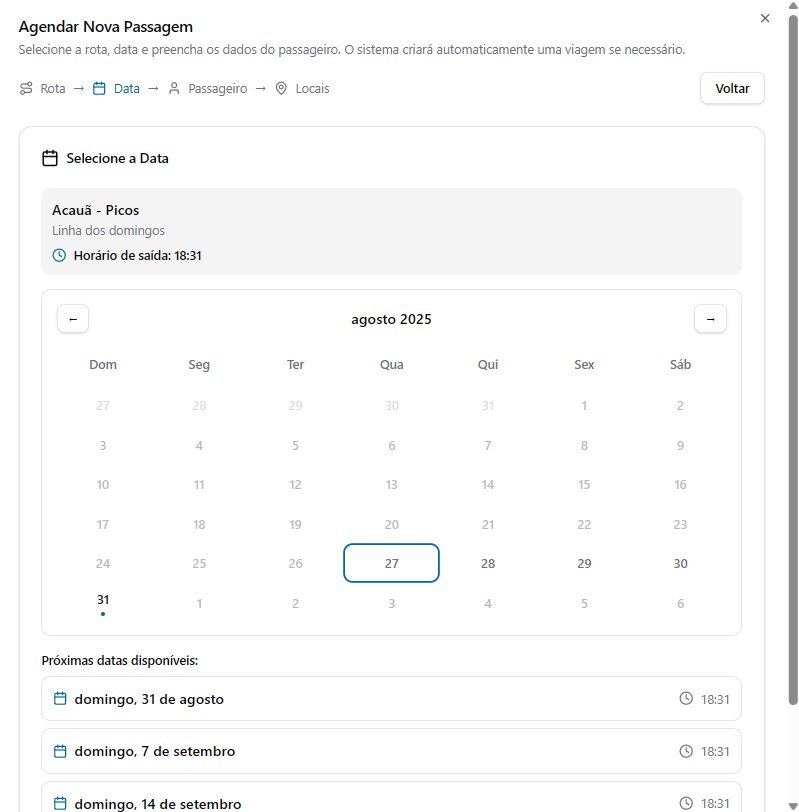
\includegraphics[width=0.9\textwidth]{imagens/wizard-data.png}
  \caption{Seleção de data e horário.}
  \label{fig:wizard-data}
\end{figure}

\subsubsection{3. Informações do Passageiro}

Terceira etapa para coleta de dados pessoais (nome completo, CPF), contatos (telefone, email) e validação automática de CPF.

\begin{figure}[H]
  \centering
  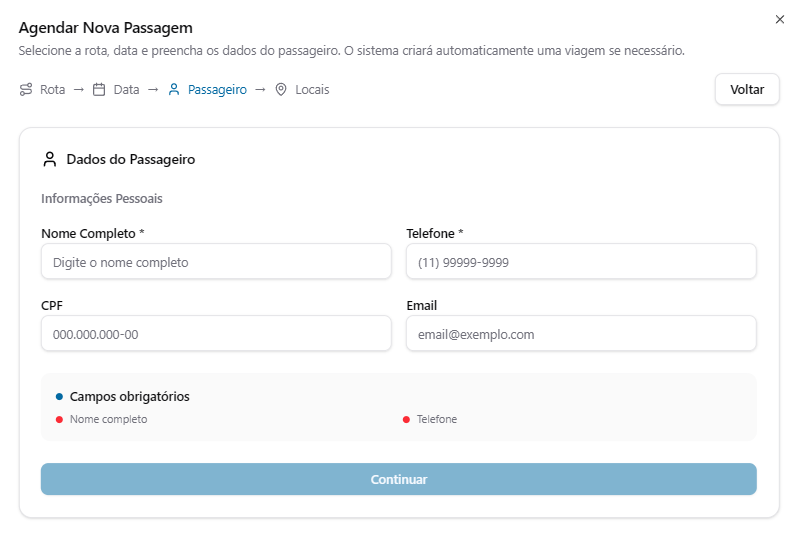
\includegraphics[width=0.9\textwidth]{imagens/wizard-passageiro.png}
  \caption{Cadastro de informações do passageiro.}
  \label{fig:wizard-passageiro}
\end{figure}

\subsubsection{4. Seleção de Locais de Embarque e Desembarque}

Quarta etapa com seleção de paradas oficiais ou definição de locais personalizados, cálculo de preço baseado na distância e observações para o motorista.

\begin{figure}[H]
  \centering
  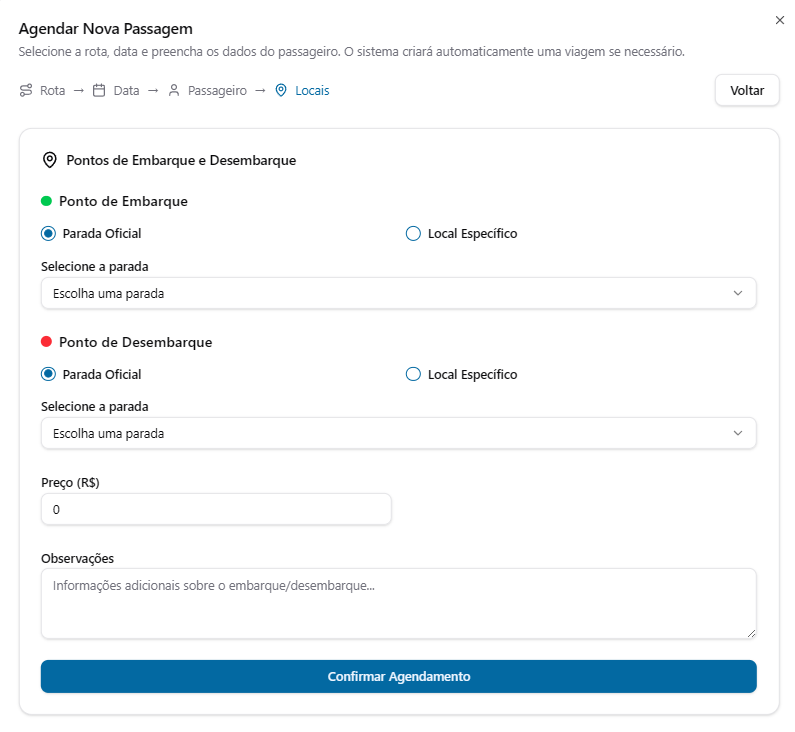
\includegraphics[width=0.9\textwidth]{imagens/wizard-locais.png}
  \caption{Seleção de locais de embarque e desembarque.}
  \label{fig:wizard-locais}
\end{figure}

\subsubsection{5. Confirmação e Pagamento}

Etapa final com resumo da viagem, detalhes da passagem, preço final e geração automática do bilhete.

\begin{figure}[H]
  \centering
  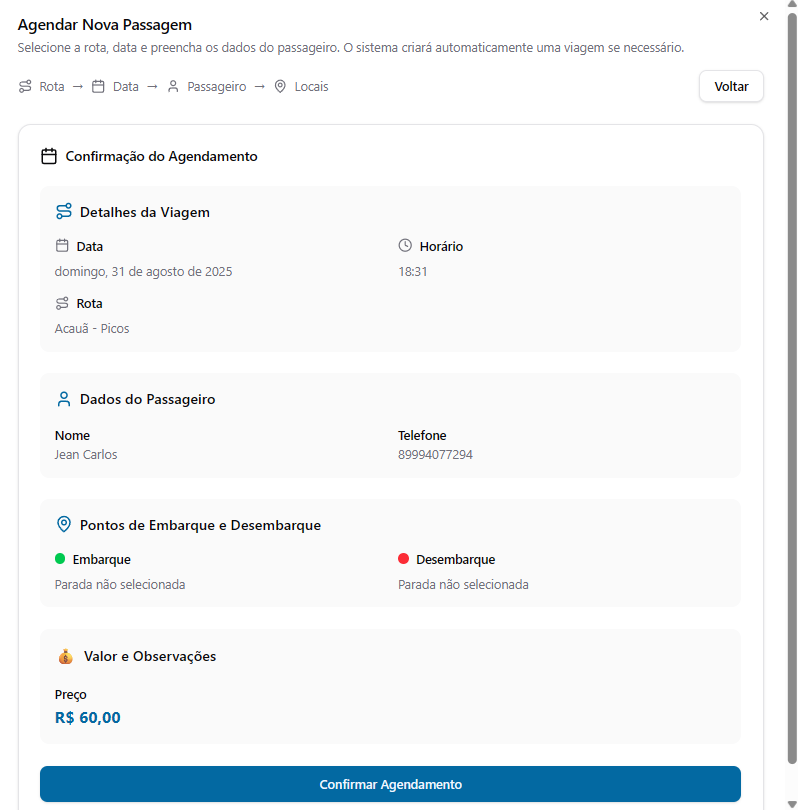
\includegraphics[width=0.9\textwidth]{imagens/wizard-confirmacao.png}
  \caption{Confirmação final e geração da passagem.}
  \label{fig:wizard-confirmacao}
\end{figure}

\section{Características da Interface}

\subsection{Design Responsivo}

A interface é totalmente responsiva, adaptando-se a diferentes tamanhos de tela: desktop com layout completo, tablet com adaptação automática e mobile com interface otimizada.

\subsection{Experiência do Usuário}

O sistema prioriza a usabilidade através de navegação intuitiva, feedback visual com notificações e estados de carregamento, validação em tempo real e suporte à acessibilidade.

\subsection{Integração com Mapas}

A integração com mapas interativos (Leaflet) oferece visualização geográfica precisa, seleção por clique, funcionalidade de arrastar e soltar para ajuste fino e controles intuitivos de zoom e navegação.

O frontend do BusLy proporciona uma experiência completa e profissional para gestão de operações de transporte, combinando funcionalidade avançada com interface intuitiva e moderna.

